\documentclass[10pt,a4paper]{article}
\usepackage[latin1]{inputenc}
\usepackage{amsmath}
\usepackage{amsfonts}
\usepackage{amssymb}
\usepackage{mathtools}
\usepackage{bm}
\usepackage{standalone}
% Use \bm{x} for vectors/matrices in bold AND italic

\newcommand{\vectornorm}[1]{\left\|#1\right\|}

\begin{document}
\section*{Verification And Convergence Analysis}
With no analytical solution available, verification of our scheme proved to be difficult. As seen from figure \ref{L2sol} the $L^2(\Omega)$-norm of our solution approaches some value around 0.006. The values attained numerically are strictly decreasing towards this value, and shows signs of convergence for our method. Figure \ref{L2error} shows the $L^2$-norm of the difference between numerically attained solutions $u_h$ and a reference solution $u_{ref}$. The reference solution is also attained numerically by using the same method, but on a much finer grid than the other solutions. The reference used in Figure \ref{L2error} is the solution attained using a mesh with 1000 points in each spatial directions. It is seen that the value is strictly decreasing as the number of points grows closer to 1000. It is clear that if we assume the reference solution to be a good approximation to the analytical solution, the method shows signs of convergence towards this solution.

\begin{figure}
    \centering
    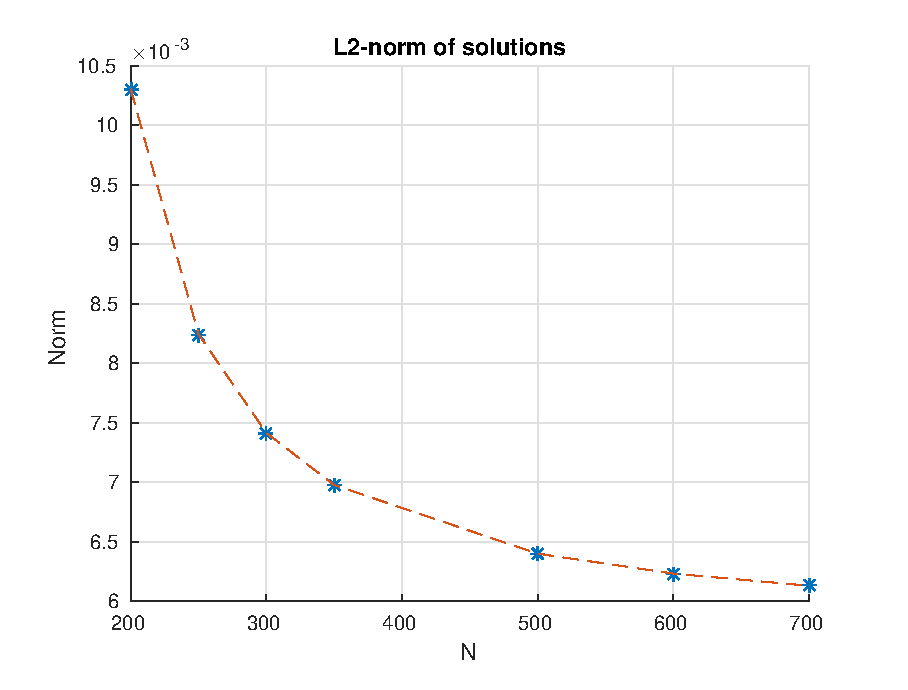
\includegraphics[scale=0.8]{figures/L2solutions}
    \caption{$\vectornorm{u_h}_{L^2(\Omega)}$ as a function of number of node points in each direction}
    \label{L2sol}
\end{figure} 

\begin{figure}
    \centering
    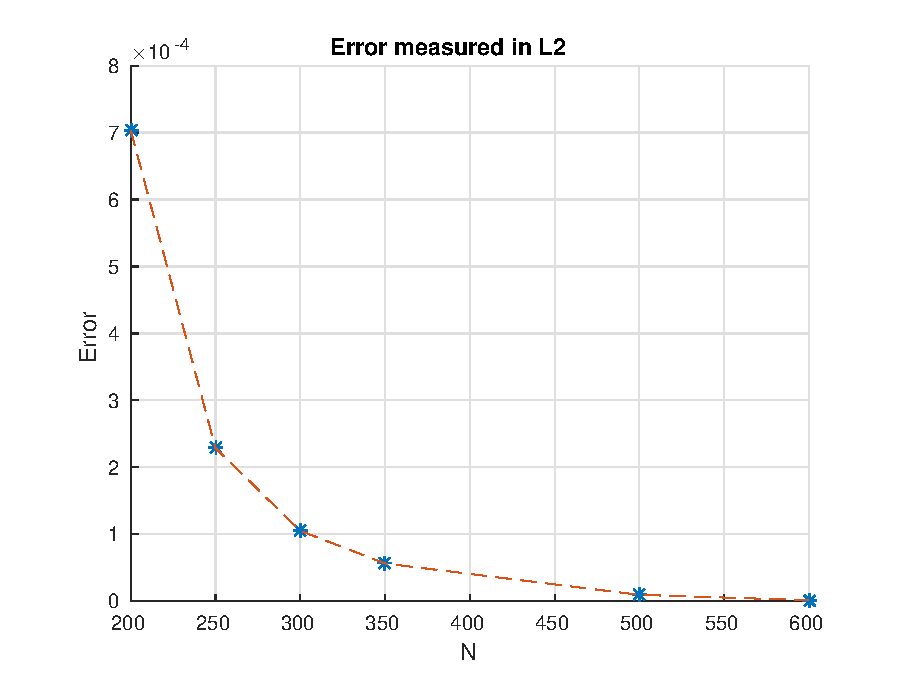
\includegraphics[scale=0.8]{figures/L2_error}
    \caption{$\vectornorm{u_{ref} - u_h}_{L^2(\Omega)}$ as a function of number of node points in each direction}
    \label{L2error}
\end{figure}


\end{document}